\documentclass{article}
\usepackage[utf8]{inputenc}
\usepackage[T1]{fontenc}
\usepackage[a4paper,total={6in,8in}]{geometry}
\usepackage{amsmath,amssymb,amsfonts}
\usepackage{graphicx}
\usepackage{hyperref}
\usepackage{enumitem}
\usepackage{listings}
\usepackage{xcolor}
\DeclareMathOperator{\Var}{Var}
\DeclareMathOperator{\Cov}{Cov}
\providecommand{\tightlist}{\setlength{\itemsep}{0pt}\setlength{\parskip}{0pt}}
\lstset{basicstyle=\ttfamily\scriptsize,breaklines=true,columns=fullflexible,
  keepspaces=true,showstringspaces=false,frame=single}
\hypersetup{colorlinks=true,urlcolor=blue,linkcolor=blue}
\setlength{\emergencystretch}{2em}

\title{Math 126 Problem 5: Hashing Around the Clock}
\author{} % Put your name here.
\date{Spring 2027}
\begin{document}
\maketitle

\hypertarget{submission-instructions}{%
\subsection*{Submission Instructions}\label{submission-instructions}}

Please upload your work to Gradescope by \textbf{11:59pm on Monday, February 8, 2027 (Pacific time).}

\begin{itemize}
\item
  You are encouraged to discuss ideas and work with your classmates. However, you \emph{must acknowledge} your collaborators at the top of each solution on which you collaborated with others and you \emph{must write} your solutions independently.
\item
  Your solutions to theory questions must be written legibly, or typeset in LaTeX or markdown.
\item
  I recommend that you write your solutions in a Python notebook using Google Colab.
\item
  You should submit your solutions as a \emph{single PDF} via the assignment on Gradescope.
\end{itemize}

\textbf{Grading:} The point of the problem set is for \emph{you} to learn. To this end, I hope to disincentivize the use of LLMs by \emph{not} grading your work for correctness. Instead, you will grade your own work by comparing it to my solutions. This self-grade is due the Friday \emph{after} the problem set is due, also on Gradescope.

\noindent Original notebook: \href{https://colab.research.google.com/drive/1LuRvgAY3ruIoxXY4w99kkiT-8luiVyo9?usp=sharing}{Google Colab}.

% Source notebook cell 2
\hypertarget{hashing-around-the-clock}{%
\subsection*{Hashing Around the Clock}\label{hashing-around-the-clock}}

In modern systems, hashing is often used to distribute data items or computational tasks to a collection of servers. What happens when a server is added or removed from a system? Most hash functions, including those discussed in class, are tailored to the number of servers, \(n\), and would change completely if \(n\) changes. This would require rehashing and moving all of our \(m\) data items, an expensive operation.

% Source notebook cell 3
\begin{center}
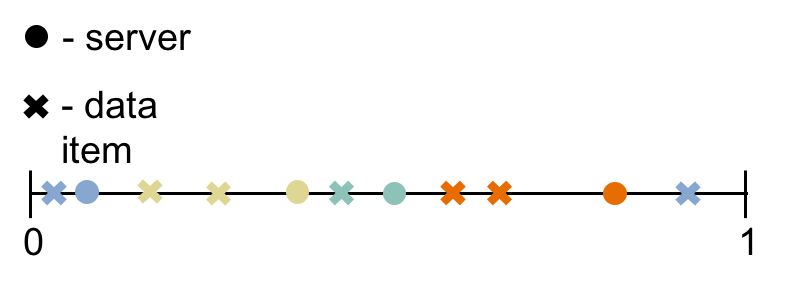
\includegraphics[width=0.65\linewidth,height=0.28\textheight,keepaspectratio]{images/problem05-figure1.png}
\end{center}

% Source notebook cell 4
Here we consider an approach to avoid this problem. Assume we have access to a completely random hash function that maps any value \(x\) to a real value \(h(x) \in [0,1]\). Use the hash function to map \emph{both} data items and servers randomly to \([0,1]\). Each data item is stored on the first server to its right on the number line (with wrap around -- i.e.~a job hashed below 1 but above all servers is assigned to the first server after 0). When a new server is added to the system, we hash it to \([0,1]\) and move data items accordingly.

% Source notebook cell 5
\hypertarget{part-a}{%
\subsection*{Part A}\label{part-a}}

Suppose we have \(n\) servers initially. When a new server is added to the system, what is the expected number of data items that need to be relocated?

% Source notebook cell 6
\hypertarget{part-b}{%
\subsection*{Part B}\label{part-b}}

Show that, with probability \(>9/10\), no server ``owns'' more than an \begin{align*}\frac{\log_e (10 n)}{n}\end{align*} fraction of the interval \([0,1]\). This can be proven \emph{without} a concentration bound.

\textbf{Hint 1:} \begin{align*}\left(1-\frac1{z}\right)^z \leq \frac1{e}\end{align*}

\end{document}
